\documentclass[twoside]{book}

% Packages required by doxygen
\usepackage{fixltx2e}
\usepackage{calc}
\usepackage{doxygen}
\usepackage[export]{adjustbox} % also loads graphicx
\usepackage{graphicx}
\usepackage[utf8]{inputenc}
\usepackage{makeidx}
\usepackage{multicol}
\usepackage{multirow}
\PassOptionsToPackage{warn}{textcomp}
\usepackage{textcomp}
\usepackage[nointegrals]{wasysym}
\usepackage[table]{xcolor}

% Font selection
\usepackage[T1]{fontenc}
\usepackage[scaled=.90]{helvet}
\usepackage{courier}
\usepackage{amssymb}
\usepackage{sectsty}
\renewcommand{\familydefault}{\sfdefault}
\allsectionsfont{%
  \fontseries{bc}\selectfont%
  \color{darkgray}%
}
\renewcommand{\DoxyLabelFont}{%
  \fontseries{bc}\selectfont%
  \color{darkgray}%
}
\newcommand{\+}{\discretionary{\mbox{\scriptsize$\hookleftarrow$}}{}{}}

% Page & text layout
\usepackage{geometry}
\geometry{%
  a4paper,%
  top=2.5cm,%
  bottom=2.5cm,%
  left=2.5cm,%
  right=2.5cm%
}
\tolerance=750
\hfuzz=15pt
\hbadness=750
\setlength{\emergencystretch}{15pt}
\setlength{\parindent}{0cm}
\setlength{\parskip}{3ex plus 2ex minus 2ex}
\makeatletter
\renewcommand{\paragraph}{%
  \@startsection{paragraph}{4}{0ex}{-1.0ex}{1.0ex}{%
    \normalfont\normalsize\bfseries\SS@parafont%
  }%
}
\renewcommand{\subparagraph}{%
  \@startsection{subparagraph}{5}{0ex}{-1.0ex}{1.0ex}{%
    \normalfont\normalsize\bfseries\SS@subparafont%
  }%
}
\makeatother

% Headers & footers
\usepackage{fancyhdr}
\pagestyle{fancyplain}
\fancyhead[LE]{\fancyplain{}{\bfseries\thepage}}
\fancyhead[CE]{\fancyplain{}{}}
\fancyhead[RE]{\fancyplain{}{\bfseries\leftmark}}
\fancyhead[LO]{\fancyplain{}{\bfseries\rightmark}}
\fancyhead[CO]{\fancyplain{}{}}
\fancyhead[RO]{\fancyplain{}{\bfseries\thepage}}
\fancyfoot[LE]{\fancyplain{}{}}
\fancyfoot[CE]{\fancyplain{}{}}
\fancyfoot[RE]{\fancyplain{}{\bfseries\scriptsize Generated by Doxygen }}
\fancyfoot[LO]{\fancyplain{}{\bfseries\scriptsize Generated by Doxygen }}
\fancyfoot[CO]{\fancyplain{}{}}
\fancyfoot[RO]{\fancyplain{}{}}
\renewcommand{\footrulewidth}{0.4pt}
\renewcommand{\chaptermark}[1]{%
  \markboth{#1}{}%
}
\renewcommand{\sectionmark}[1]{%
  \markright{\thesection\ #1}%
}

% Indices & bibliography
\usepackage{natbib}
\usepackage[titles]{tocloft}
\setcounter{tocdepth}{3}
\setcounter{secnumdepth}{5}
\makeindex

% Hyperlinks (required, but should be loaded last)
\usepackage{ifpdf}
\ifpdf
  \usepackage[pdftex,pagebackref=true]{hyperref}
\else
  \usepackage[ps2pdf,pagebackref=true]{hyperref}
\fi
\hypersetup{%
  colorlinks=true,%
  linkcolor=blue,%
  citecolor=blue,%
  unicode%
}

% Custom commands
\newcommand{\clearemptydoublepage}{%
  \newpage{\pagestyle{empty}\cleardoublepage}%
}

\usepackage{caption}
\captionsetup{labelsep=space,justification=centering,font={bf},singlelinecheck=off,skip=4pt,position=top}

%===== C O N T E N T S =====

\begin{document}

% Titlepage & ToC
\hypersetup{pageanchor=false,
             bookmarksnumbered=true,
             pdfencoding=unicode
            }
\pagenumbering{alph}
\begin{titlepage}
\vspace*{7cm}
\begin{center}%
{\Large Liquid\+\_\+\+Project3 }\\
\vspace*{1cm}
{\large Generated by Doxygen 1.8.13}\\
\end{center}
\end{titlepage}
\clearemptydoublepage
\pagenumbering{roman}
\tableofcontents
\clearemptydoublepage
\pagenumbering{arabic}
\hypersetup{pageanchor=true}

%--- Begin generated contents ---
\chapter{Hierarchical Index}
\section{Class Hierarchy}
This inheritance list is sorted roughly, but not completely, alphabetically\+:\begin{DoxyCompactList}
\item \contentsline{section}{Game\+Logic}{\pageref{class_game_logic}}{}
\item Mono\+Behaviour\begin{DoxyCompactList}
\item \contentsline{section}{Ability\+Control1}{\pageref{class_ability_control1}}{}
\item \contentsline{section}{Ability\+Use}{\pageref{class_ability_use}}{}
\item \contentsline{section}{Animation\+Events}{\pageref{class_animation_events}}{}
\item \contentsline{section}{Click\+To\+Move}{\pageref{class_click_to_move}}{}
\item \contentsline{section}{enemy\+\_\+movement}{\pageref{classenemy__movement}}{}
\item \contentsline{section}{Enemy\+Controller}{\pageref{class_enemy_controller}}{}
\item \contentsline{section}{Fire\+Ball\+Ability}{\pageref{class_fire_ball_ability}}{}
\item \contentsline{section}{Fire\+Ball\+Destroy}{\pageref{class_fire_ball_destroy}}{}
\item \contentsline{section}{Menu\+Button}{\pageref{class_menu_button}}{}
\item \contentsline{section}{Player\+Controller}{\pageref{class_player_controller}}{}
\item \contentsline{section}{U\+I\+Controller}{\pageref{class_u_i_controller}}{}
\item \contentsline{section}{wave\+\_\+spawner}{\pageref{classwave__spawner}}{}
\item \contentsline{section}{waypoints}{\pageref{classwaypoints}}{}
\end{DoxyCompactList}
\end{DoxyCompactList}

\chapter{Class Index}
\section{Class List}
Here are the classes, structs, unions and interfaces with brief descriptions\+:\begin{DoxyCompactList}
\item\contentsline{section}{\hyperlink{class_ability_control1}{Ability\+Control1} }{\pageref{class_ability_control1}}{}
\item\contentsline{section}{\hyperlink{class_ability_use}{Ability\+Use} }{\pageref{class_ability_use}}{}
\item\contentsline{section}{\hyperlink{class_animation_events}{Animation\+Events} }{\pageref{class_animation_events}}{}
\item\contentsline{section}{\hyperlink{class_click_to_move}{Click\+To\+Move} }{\pageref{class_click_to_move}}{}
\item\contentsline{section}{\hyperlink{classenemy__movement}{enemy\+\_\+movement} }{\pageref{classenemy__movement}}{}
\item\contentsline{section}{\hyperlink{class_enemy_controller}{Enemy\+Controller} }{\pageref{class_enemy_controller}}{}
\item\contentsline{section}{\hyperlink{class_fire_ball_ability}{Fire\+Ball\+Ability} }{\pageref{class_fire_ball_ability}}{}
\item\contentsline{section}{\hyperlink{class_fire_ball_destroy}{Fire\+Ball\+Destroy} }{\pageref{class_fire_ball_destroy}}{}
\item\contentsline{section}{\hyperlink{class_game_logic}{Game\+Logic} }{\pageref{class_game_logic}}{}
\item\contentsline{section}{\hyperlink{class_menu_button}{Menu\+Button} }{\pageref{class_menu_button}}{}
\item\contentsline{section}{\hyperlink{class_player_controller}{Player\+Controller} }{\pageref{class_player_controller}}{}
\item\contentsline{section}{\hyperlink{class_u_i_controller}{U\+I\+Controller} }{\pageref{class_u_i_controller}}{}
\item\contentsline{section}{\hyperlink{classwave__spawner}{wave\+\_\+spawner} }{\pageref{classwave__spawner}}{}
\item\contentsline{section}{\hyperlink{classwaypoints}{waypoints} }{\pageref{classwaypoints}}{}
\end{DoxyCompactList}

\chapter{Class Documentation}
\hypertarget{class_click_to_move}{}\section{Click\+To\+Move Class Reference}
\label{class_click_to_move}\index{Click\+To\+Move@{Click\+To\+Move}}
Inheritance diagram for Click\+To\+Move\+:\begin{figure}[H]
\begin{center}
\leavevmode
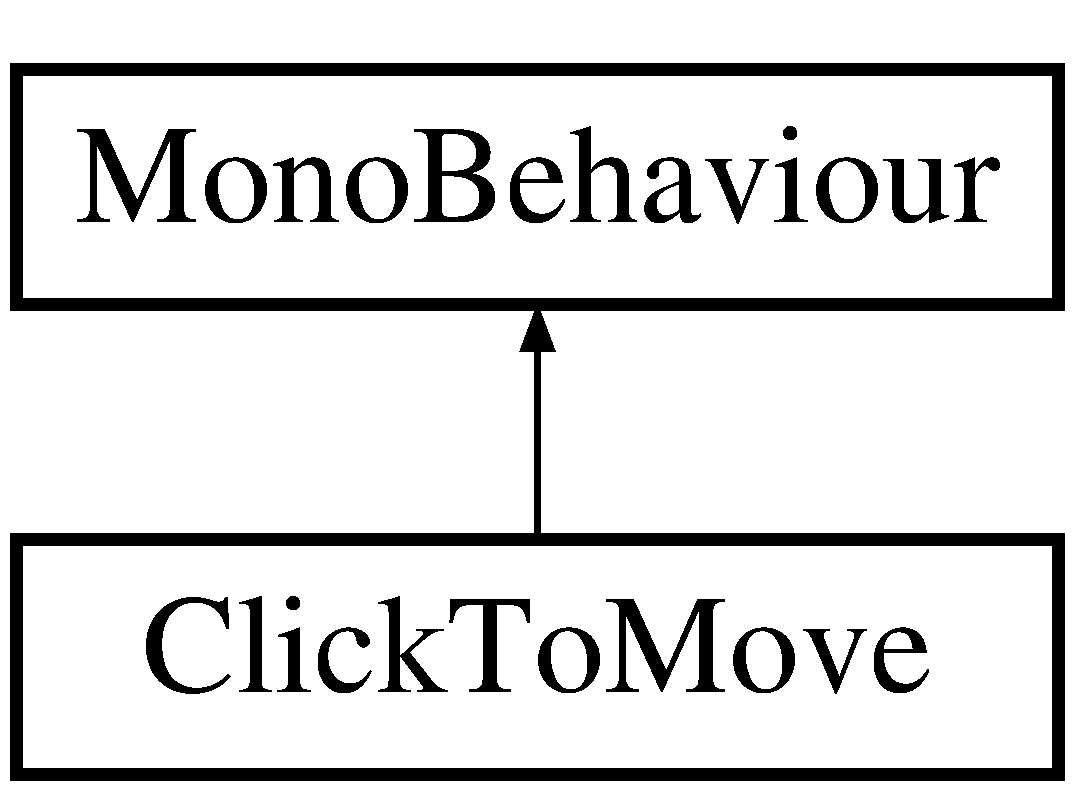
\includegraphics[height=2.000000cm]{class_click_to_move}
\end{center}
\end{figure}
\subsection*{Public Attributes}
\begin{DoxyCompactItemize}
\item 
\mbox{\Hypertarget{class_click_to_move_aac470519ddd58c7abd2483189fad68a1}\label{class_click_to_move_aac470519ddd58c7abd2483189fad68a1}} 
float {\bfseries speed}
\item 
\mbox{\Hypertarget{class_click_to_move_ad53ee05cf310c30384135105872ba4ec}\label{class_click_to_move_ad53ee05cf310c30384135105872ba4ec}} 
float {\bfseries attacktime}
\item 
\mbox{\Hypertarget{class_click_to_move_a994f7ef477344b83f88a2e3f6cc851d7}\label{class_click_to_move_a994f7ef477344b83f88a2e3f6cc851d7}} 
Character\+Controller {\bfseries controller}
\item 
\mbox{\Hypertarget{class_click_to_move_ac94045aa2258a65663f2a808253d5aa5}\label{class_click_to_move_ac94045aa2258a65663f2a808253d5aa5}} 
Animator {\bfseries anim}
\item 
\mbox{\Hypertarget{class_click_to_move_a8268ad4762bb2f7487c71036e269bde4}\label{class_click_to_move_a8268ad4762bb2f7487c71036e269bde4}} 
float {\bfseries attack\+Damage}
\item 
\mbox{\Hypertarget{class_click_to_move_ad66cd916848620bfecd80b52c4a9511a}\label{class_click_to_move_ad66cd916848620bfecd80b52c4a9511a}} 
float {\bfseries attack\+Speed}
\item 
\mbox{\Hypertarget{class_click_to_move_a5f4d06a67a3c86936fe45943e52d6b94}\label{class_click_to_move_a5f4d06a67a3c86936fe45943e52d6b94}} 
float {\bfseries attack\+Range}
\end{DoxyCompactItemize}
\subsection*{Static Public Attributes}
\begin{DoxyCompactItemize}
\item 
\mbox{\Hypertarget{class_click_to_move_a1c210864eeb2d4b60b6ca933b0aa6b2d}\label{class_click_to_move_a1c210864eeb2d4b60b6ca933b0aa6b2d}} 
static bool {\bfseries attack}
\item 
\mbox{\Hypertarget{class_click_to_move_a263b8d7596f06f4c3cfa4219f1c728cc}\label{class_click_to_move_a263b8d7596f06f4c3cfa4219f1c728cc}} 
static bool {\bfseries die}
\end{DoxyCompactItemize}
\subsection*{Private Member Functions}
\begin{DoxyCompactItemize}
\item 
void \hyperlink{class_click_to_move_ab5f10418f80164154a69d18809fec30d}{Start} ()
\item 
void \hyperlink{class_click_to_move_aa9c5f267b0b5ad54a2444aaddec00862}{Update} ()
\item 
void \hyperlink{class_click_to_move_ad8ff402015f7fb9e9e850400ca47e47b}{locate\+Position} ()
\item 
void \hyperlink{class_click_to_move_add7581013c28bc5180a4111a196cec41}{move\+To\+Position} ()
\item 
void \hyperlink{class_click_to_move_a7a22f9529f61a4da097d950d65b5bcaa}{Attack} ()
\item 
I\+Enumerator \hyperlink{class_click_to_move_a81c5db2ca3553c2bb0cd6473437a5561}{Attack\+Routine} ()
\item 
I\+Enumerator \hyperlink{class_click_to_move_a9ec6685677f20e880a600762dd64d22a}{Attack\+Cooldown} ()
\item 
void \hyperlink{class_click_to_move_a12f6a353fabc43f592dd239da275b5e6}{Get\+Enemies\+In\+Range} ()
\end{DoxyCompactItemize}
\subsection*{Private Attributes}
\begin{DoxyCompactItemize}
\item 
\mbox{\Hypertarget{class_click_to_move_afd98b037b9175c78885ad6a7815a11b8}\label{class_click_to_move_afd98b037b9175c78885ad6a7815a11b8}} 
Vector3 {\bfseries position}
\item 
\mbox{\Hypertarget{class_click_to_move_aa1b653d4efebd28d2a2b644e2bc5abb7}\label{class_click_to_move_aa1b653d4efebd28d2a2b644e2bc5abb7}} 
List$<$ Transform $>$ {\bfseries enemies\+In\+Range} = new List$<$Transform$>$ ()
\item 
\mbox{\Hypertarget{class_click_to_move_acad5001efecf12cd5a0e326bbab8b6c8}\label{class_click_to_move_acad5001efecf12cd5a0e326bbab8b6c8}} 
bool {\bfseries can\+Move}
\item 
\mbox{\Hypertarget{class_click_to_move_ae7968592257870641fce73765fda4c12}\label{class_click_to_move_ae7968592257870641fce73765fda4c12}} 
bool {\bfseries can\+Attack}
\end{DoxyCompactItemize}


\subsection{Member Function Documentation}
\mbox{\Hypertarget{class_click_to_move_a7a22f9529f61a4da097d950d65b5bcaa}\label{class_click_to_move_a7a22f9529f61a4da097d950d65b5bcaa}} 
\index{Click\+To\+Move@{Click\+To\+Move}!Attack@{Attack}}
\index{Attack@{Attack}!Click\+To\+Move@{Click\+To\+Move}}
\subsubsection{\texorpdfstring{Attack()}{Attack()}}
{\footnotesize\ttfamily void Click\+To\+Move.\+Attack (\begin{DoxyParamCaption}{ }\end{DoxyParamCaption})\hspace{0.3cm}{\ttfamily [private]}}

Pre\+: player object created and attack key is pressed Post\+: animation of attacking called return\+: NA \mbox{\Hypertarget{class_click_to_move_a9ec6685677f20e880a600762dd64d22a}\label{class_click_to_move_a9ec6685677f20e880a600762dd64d22a}} 
\index{Click\+To\+Move@{Click\+To\+Move}!Attack\+Cooldown@{Attack\+Cooldown}}
\index{Attack\+Cooldown@{Attack\+Cooldown}!Click\+To\+Move@{Click\+To\+Move}}
\subsubsection{\texorpdfstring{Attack\+Cooldown()}{AttackCooldown()}}
{\footnotesize\ttfamily I\+Enumerator Click\+To\+Move.\+Attack\+Cooldown (\begin{DoxyParamCaption}{ }\end{DoxyParamCaption})\hspace{0.3cm}{\ttfamily [private]}}

Pre\+: player object created Post\+: attack animation cooldown set/adjusted return\+: NA \mbox{\Hypertarget{class_click_to_move_a81c5db2ca3553c2bb0cd6473437a5561}\label{class_click_to_move_a81c5db2ca3553c2bb0cd6473437a5561}} 
\index{Click\+To\+Move@{Click\+To\+Move}!Attack\+Routine@{Attack\+Routine}}
\index{Attack\+Routine@{Attack\+Routine}!Click\+To\+Move@{Click\+To\+Move}}
\subsubsection{\texorpdfstring{Attack\+Routine()}{AttackRoutine()}}
{\footnotesize\ttfamily I\+Enumerator Click\+To\+Move.\+Attack\+Routine (\begin{DoxyParamCaption}{ }\end{DoxyParamCaption})\hspace{0.3cm}{\ttfamily [private]}}

Pre\+: player object created and attack animation called Post\+: attack animation commences return\+: NA \mbox{\Hypertarget{class_click_to_move_a12f6a353fabc43f592dd239da275b5e6}\label{class_click_to_move_a12f6a353fabc43f592dd239da275b5e6}} 
\index{Click\+To\+Move@{Click\+To\+Move}!Get\+Enemies\+In\+Range@{Get\+Enemies\+In\+Range}}
\index{Get\+Enemies\+In\+Range@{Get\+Enemies\+In\+Range}!Click\+To\+Move@{Click\+To\+Move}}
\subsubsection{\texorpdfstring{Get\+Enemies\+In\+Range()}{GetEnemiesInRange()}}
{\footnotesize\ttfamily void Click\+To\+Move.\+Get\+Enemies\+In\+Range (\begin{DoxyParamCaption}{ }\end{DoxyParamCaption})\hspace{0.3cm}{\ttfamily [private]}}

Pre\+: player object created Post\+: enemy object within range is set to able to be attacked return\+: NA \mbox{\Hypertarget{class_click_to_move_ad8ff402015f7fb9e9e850400ca47e47b}\label{class_click_to_move_ad8ff402015f7fb9e9e850400ca47e47b}} 
\index{Click\+To\+Move@{Click\+To\+Move}!locate\+Position@{locate\+Position}}
\index{locate\+Position@{locate\+Position}!Click\+To\+Move@{Click\+To\+Move}}
\subsubsection{\texorpdfstring{locate\+Position()}{locatePosition()}}
{\footnotesize\ttfamily void Click\+To\+Move.\+locate\+Position (\begin{DoxyParamCaption}{ }\end{DoxyParamCaption})\hspace{0.3cm}{\ttfamily [private]}}

Pre\+: player object created Post\+: position of enemy determined for attack return\+: NA \mbox{\Hypertarget{class_click_to_move_add7581013c28bc5180a4111a196cec41}\label{class_click_to_move_add7581013c28bc5180a4111a196cec41}} 
\index{Click\+To\+Move@{Click\+To\+Move}!move\+To\+Position@{move\+To\+Position}}
\index{move\+To\+Position@{move\+To\+Position}!Click\+To\+Move@{Click\+To\+Move}}
\subsubsection{\texorpdfstring{move\+To\+Position()}{moveToPosition()}}
{\footnotesize\ttfamily void Click\+To\+Move.\+move\+To\+Position (\begin{DoxyParamCaption}{ }\end{DoxyParamCaption})\hspace{0.3cm}{\ttfamily [private]}}

Pre\+: player object created Post\+: player moved to position of click return\+: NA \mbox{\Hypertarget{class_click_to_move_ab5f10418f80164154a69d18809fec30d}\label{class_click_to_move_ab5f10418f80164154a69d18809fec30d}} 
\index{Click\+To\+Move@{Click\+To\+Move}!Start@{Start}}
\index{Start@{Start}!Click\+To\+Move@{Click\+To\+Move}}
\subsubsection{\texorpdfstring{Start()}{Start()}}
{\footnotesize\ttfamily void Click\+To\+Move.\+Start (\begin{DoxyParamCaption}{ }\end{DoxyParamCaption})\hspace{0.3cm}{\ttfamily [private]}}

Pre\+: player object created Post\+: player object initialized to allow for movement and attack return\+: NA \mbox{\Hypertarget{class_click_to_move_aa9c5f267b0b5ad54a2444aaddec00862}\label{class_click_to_move_aa9c5f267b0b5ad54a2444aaddec00862}} 
\index{Click\+To\+Move@{Click\+To\+Move}!Update@{Update}}
\index{Update@{Update}!Click\+To\+Move@{Click\+To\+Move}}
\subsubsection{\texorpdfstring{Update()}{Update()}}
{\footnotesize\ttfamily void Click\+To\+Move.\+Update (\begin{DoxyParamCaption}{ }\end{DoxyParamCaption})\hspace{0.3cm}{\ttfamily [private]}}

Pre\+: player object created Post\+: methods called as based on input of mouse or keyboard return\+: NA 

The documentation for this class was generated from the following file\+:\begin{DoxyCompactItemize}
\item 
F\+:/\+E\+E\+C\+S448/project3/\+Project3/3\+D-\/\+R\+P\+G/\+Assets/\+Scripts/Click\+To\+Move.\+cs\end{DoxyCompactItemize}

\hypertarget{classenemy__movement}{}\section{enemy\+\_\+movement Class Reference}
\label{classenemy__movement}\index{enemy\+\_\+movement@{enemy\+\_\+movement}}
Inheritance diagram for enemy\+\_\+movement\+:\begin{figure}[H]
\begin{center}
\leavevmode
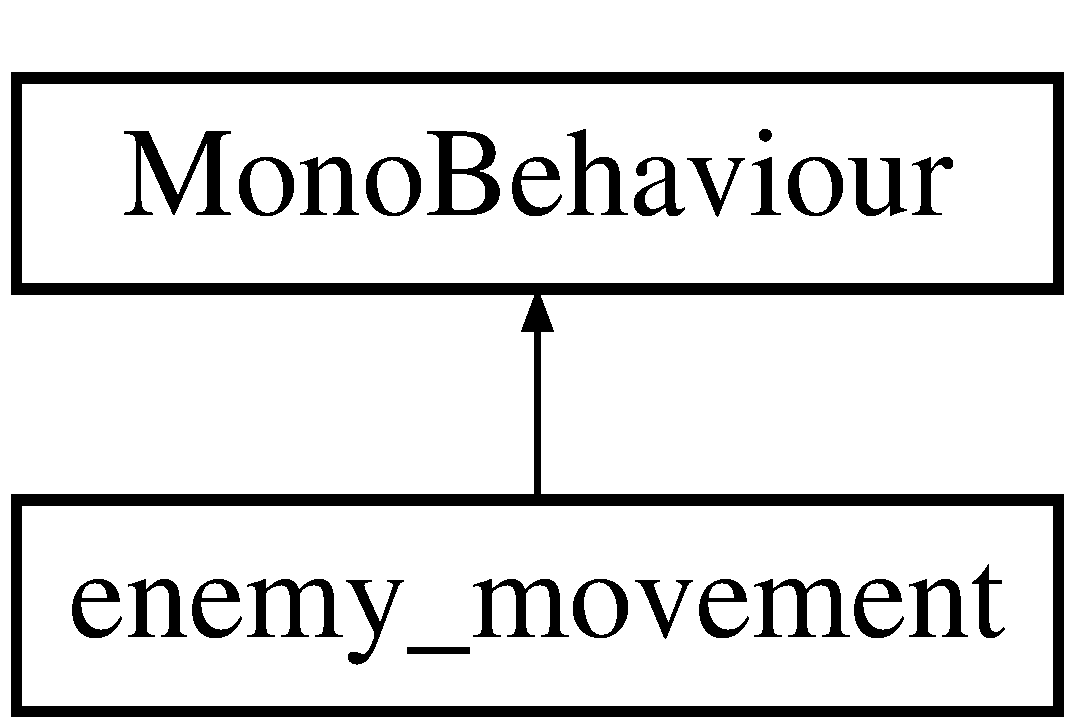
\includegraphics[height=2.000000cm]{classenemy__movement}
\end{center}
\end{figure}
\subsection*{Public Attributes}
\begin{DoxyCompactItemize}
\item 
\mbox{\Hypertarget{classenemy__movement_aaa269754d38c16dcce632cafebb2e370}\label{classenemy__movement_aaa269754d38c16dcce632cafebb2e370}} 
float {\bfseries enemy\+\_\+speed} = 10f
\item 
\mbox{\Hypertarget{classenemy__movement_a45601a45a3c6ff8a8566fe3fe8924991}\label{classenemy__movement_a45601a45a3c6ff8a8566fe3fe8924991}} 
float {\bfseries attack\+Damage}
\item 
\mbox{\Hypertarget{classenemy__movement_ac5fd26c4fa810e357a52251b25f31805}\label{classenemy__movement_ac5fd26c4fa810e357a52251b25f31805}} 
int {\bfseries testing} = 0
\end{DoxyCompactItemize}
\subsection*{Private Member Functions}
\begin{DoxyCompactItemize}
\item 
void \hyperlink{classenemy__movement_a6f78b4e6952786e1ee8d7063b4c59dba}{Start} ()
\item 
void \hyperlink{classenemy__movement_a6937591e8d99aec470f81199b0850967}{Update} ()
\end{DoxyCompactItemize}
\subsection*{Private Attributes}
\begin{DoxyCompactItemize}
\item 
\mbox{\Hypertarget{classenemy__movement_a21eb53aeae43e83264e5a567dae3382b}\label{classenemy__movement_a21eb53aeae43e83264e5a567dae3382b}} 
Transform {\bfseries target}
\item 
\mbox{\Hypertarget{classenemy__movement_aeb8340df38b3b6e8d8974fd3ddc1de07}\label{classenemy__movement_aeb8340df38b3b6e8d8974fd3ddc1de07}} 
int {\bfseries wavepiont\+\_\+index} = 0
\item 
\mbox{\Hypertarget{classenemy__movement_a5040f773cb0da2de57c204fae8f8d37d}\label{classenemy__movement_a5040f773cb0da2de57c204fae8f8d37d}} 
Text {\bfseries enemy\+\_\+death\+\_\+test\+\_\+text}
\item 
\mbox{\Hypertarget{classenemy__movement_ac9c8c31e0c99bad28b5d788a165ed40c}\label{classenemy__movement_ac9c8c31e0c99bad28b5d788a165ed40c}} 
Game\+Object \mbox{[}$\,$\mbox{]} {\bfseries players}
\end{DoxyCompactItemize}


\subsection{Member Function Documentation}
\mbox{\Hypertarget{classenemy__movement_a6f78b4e6952786e1ee8d7063b4c59dba}\label{classenemy__movement_a6f78b4e6952786e1ee8d7063b4c59dba}} 
\index{enemy\+\_\+movement@{enemy\+\_\+movement}!Start@{Start}}
\index{Start@{Start}!enemy\+\_\+movement@{enemy\+\_\+movement}}
\subsubsection{\texorpdfstring{Start()}{Start()}}
{\footnotesize\ttfamily void enemy\+\_\+movement.\+Start (\begin{DoxyParamCaption}{ }\end{DoxyParamCaption})\hspace{0.3cm}{\ttfamily [private]}}

Pre\+: enemy object created Post\+: enemy object initialized by setting target to the first waypoint return\+: NA \mbox{\Hypertarget{classenemy__movement_a6937591e8d99aec470f81199b0850967}\label{classenemy__movement_a6937591e8d99aec470f81199b0850967}} 
\index{enemy\+\_\+movement@{enemy\+\_\+movement}!Update@{Update}}
\index{Update@{Update}!enemy\+\_\+movement@{enemy\+\_\+movement}}
\subsubsection{\texorpdfstring{Update()}{Update()}}
{\footnotesize\ttfamily void enemy\+\_\+movement.\+Update (\begin{DoxyParamCaption}{ }\end{DoxyParamCaption})\hspace{0.3cm}{\ttfamily [private]}}

Pre\+: enemy object initialized and has target Post\+: enemy moves towards waypoint return\+: NA 

The documentation for this class was generated from the following file\+:\begin{DoxyCompactItemize}
\item 
F\+:/\+E\+E\+C\+S448/project3/\+Project3/3\+D-\/\+R\+P\+G/\+Assets/\+Scripts/enemy\+\_\+movement.\+cs\end{DoxyCompactItemize}

\hypertarget{class_enemy_controller}{}\section{Enemy\+Controller Class Reference}
\label{class_enemy_controller}\index{Enemy\+Controller@{Enemy\+Controller}}
Inheritance diagram for Enemy\+Controller\+:\begin{figure}[H]
\begin{center}
\leavevmode
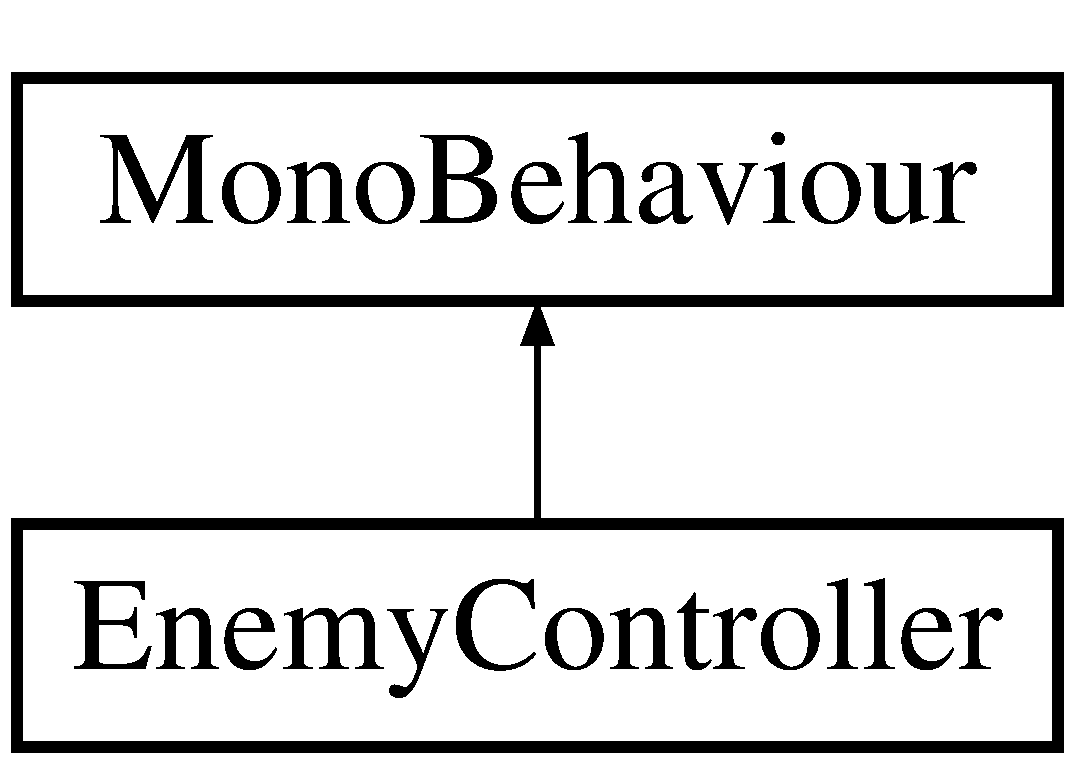
\includegraphics[height=2.000000cm]{class_enemy_controller}
\end{center}
\end{figure}
\subsection*{Public Member Functions}
\begin{DoxyCompactItemize}
\item 
void \hyperlink{class_enemy_controller_a1aefc89669c41a6353ecf463c937af07}{Get\+Hit} (float damage)
\end{DoxyCompactItemize}
\subsection*{Public Attributes}
\begin{DoxyCompactItemize}
\item 
\mbox{\Hypertarget{class_enemy_controller_a5c91ac8bc0f622901cb7a48ba787f0bd}\label{class_enemy_controller_a5c91ac8bc0f622901cb7a48ba787f0bd}} 
float {\bfseries total\+Health}
\item 
\mbox{\Hypertarget{class_enemy_controller_a7af1c6ac310289274ab51a7c2893fa0b}\label{class_enemy_controller_a7af1c6ac310289274ab51a7c2893fa0b}} 
float {\bfseries current\+Health}
\item 
\mbox{\Hypertarget{class_enemy_controller_ae505ed595e6b9807cddd599a50c55ad9}\label{class_enemy_controller_ae505ed595e6b9807cddd599a50c55ad9}} 
float {\bfseries exp\+Granted}
\item 
\mbox{\Hypertarget{class_enemy_controller_a181f04ac7727efc9ee6d200ad19b0518}\label{class_enemy_controller_a181f04ac7727efc9ee6d200ad19b0518}} 
float {\bfseries die\+Aftertime}
\end{DoxyCompactItemize}
\subsection*{Private Member Functions}
\begin{DoxyCompactItemize}
\item 
void \hyperlink{class_enemy_controller_aef5af22782327b22749e5632ad7467fb}{Start} ()
\item 
void \hyperlink{class_enemy_controller_aa2585b33cdd57288a0c5a669f188f6ca}{Die} ()
\item 
void \hyperlink{class_enemy_controller_a98b4f2b8c651189ef6b419e6400abc36}{Drop\+Loot} ()
\end{DoxyCompactItemize}
\subsection*{Private Attributes}
\begin{DoxyCompactItemize}
\item 
\mbox{\Hypertarget{class_enemy_controller_a2428b11f3cec6e784f7982b60fcc0147}\label{class_enemy_controller_a2428b11f3cec6e784f7982b60fcc0147}} 
bool {\bfseries dead}
\item 
\mbox{\Hypertarget{class_enemy_controller_a6377a2b1989ecfdde0904d0ef5d9af0a}\label{class_enemy_controller_a6377a2b1989ecfdde0904d0ef5d9af0a}} 
Game\+Object \mbox{[}$\,$\mbox{]} {\bfseries players}
\end{DoxyCompactItemize}


\subsection{Member Function Documentation}
\mbox{\Hypertarget{class_enemy_controller_aa2585b33cdd57288a0c5a669f188f6ca}\label{class_enemy_controller_aa2585b33cdd57288a0c5a669f188f6ca}} 
\index{Enemy\+Controller@{Enemy\+Controller}!Die@{Die}}
\index{Die@{Die}!Enemy\+Controller@{Enemy\+Controller}}
\subsubsection{\texorpdfstring{Die()}{Die()}}
{\footnotesize\ttfamily void Enemy\+Controller.\+Die (\begin{DoxyParamCaption}{ }\end{DoxyParamCaption})\hspace{0.3cm}{\ttfamily [private]}}

Pre\+: \hyperlink{class_enemy_controller}{Enemy\+Controller} object has no health Post\+: Enemy object destroyed return\+: NA \mbox{\Hypertarget{class_enemy_controller_a98b4f2b8c651189ef6b419e6400abc36}\label{class_enemy_controller_a98b4f2b8c651189ef6b419e6400abc36}} 
\index{Enemy\+Controller@{Enemy\+Controller}!Drop\+Loot@{Drop\+Loot}}
\index{Drop\+Loot@{Drop\+Loot}!Enemy\+Controller@{Enemy\+Controller}}
\subsubsection{\texorpdfstring{Drop\+Loot()}{DropLoot()}}
{\footnotesize\ttfamily void Enemy\+Controller.\+Drop\+Loot (\begin{DoxyParamCaption}{ }\end{DoxyParamCaption})\hspace{0.3cm}{\ttfamily [private]}}

Pre\+: Enemy object destroyed Post\+: Message printed return\+: NA \mbox{\Hypertarget{class_enemy_controller_a1aefc89669c41a6353ecf463c937af07}\label{class_enemy_controller_a1aefc89669c41a6353ecf463c937af07}} 
\index{Enemy\+Controller@{Enemy\+Controller}!Get\+Hit@{Get\+Hit}}
\index{Get\+Hit@{Get\+Hit}!Enemy\+Controller@{Enemy\+Controller}}
\subsubsection{\texorpdfstring{Get\+Hit()}{GetHit()}}
{\footnotesize\ttfamily void Enemy\+Controller.\+Get\+Hit (\begin{DoxyParamCaption}\item[{float}]{damage }\end{DoxyParamCaption})}

Pre\+: \hyperlink{class_enemy_controller}{Enemy\+Controller} object initialized and hit Post\+: \hyperlink{class_enemy_controller}{Enemy\+Controller} health adjusted return\+: NA \mbox{\Hypertarget{class_enemy_controller_aef5af22782327b22749e5632ad7467fb}\label{class_enemy_controller_aef5af22782327b22749e5632ad7467fb}} 
\index{Enemy\+Controller@{Enemy\+Controller}!Start@{Start}}
\index{Start@{Start}!Enemy\+Controller@{Enemy\+Controller}}
\subsubsection{\texorpdfstring{Start()}{Start()}}
{\footnotesize\ttfamily void Enemy\+Controller.\+Start (\begin{DoxyParamCaption}{ }\end{DoxyParamCaption})\hspace{0.3cm}{\ttfamily [private]}}

Pre\+: \hyperlink{class_enemy_controller}{Enemy\+Controller} object created Post\+: \hyperlink{class_enemy_controller}{Enemy\+Controller} object initialized return\+: NA 

The documentation for this class was generated from the following file\+:\begin{DoxyCompactItemize}
\item 
F\+:/\+E\+E\+C\+S448/project3/\+Project3/3\+D-\/\+R\+P\+G/\+Assets/\+Scripts/Enemy\+Controller.\+cs\end{DoxyCompactItemize}

\hypertarget{class_player_controller}{}\section{Player\+Controller Class Reference}
\label{class_player_controller}\index{Player\+Controller@{Player\+Controller}}
Inheritance diagram for Player\+Controller\+:\begin{figure}[H]
\begin{center}
\leavevmode
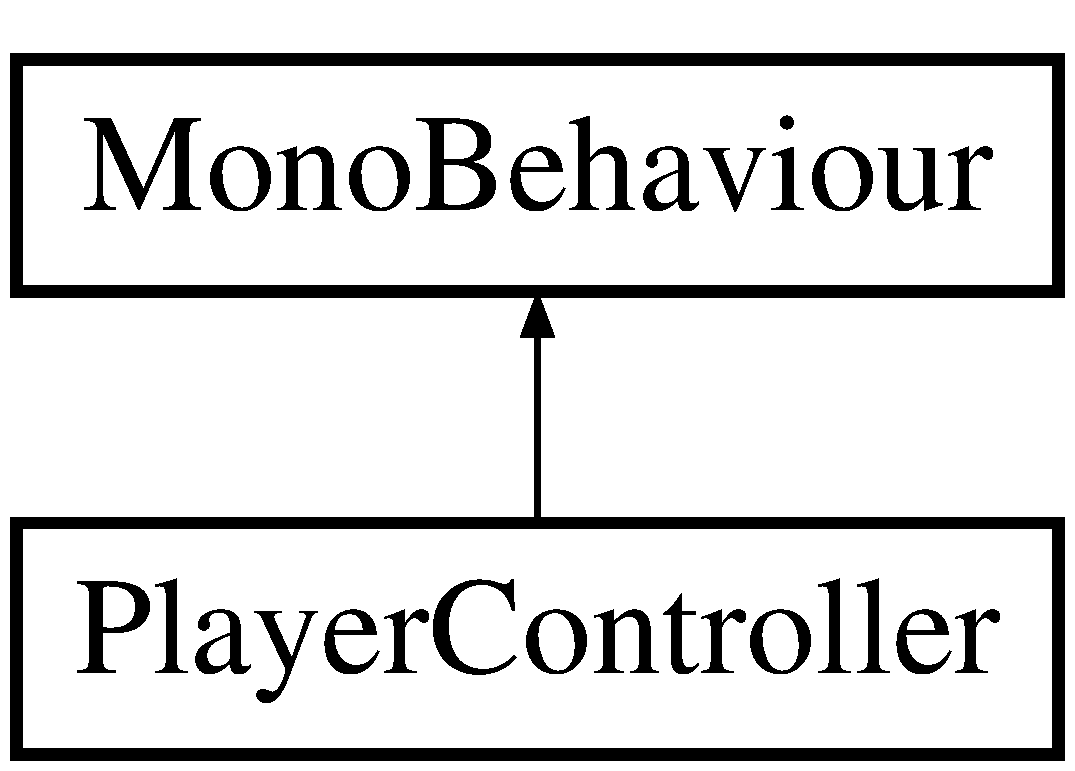
\includegraphics[height=2.000000cm]{class_player_controller}
\end{center}
\end{figure}
\subsection*{Public Member Functions}
\begin{DoxyCompactItemize}
\item 
void \hyperlink{class_player_controller_a14434c4f065a70cceb5534243df61b2b}{Set\+Experience} (float exp)
\item 
void \hyperlink{class_player_controller_a73a0a3a2d932a17798ab34abd7e885f4}{Get\+Hit} (float damage)
\item 
\mbox{\Hypertarget{class_player_controller_af91f8bb70965e0c19065950f7cbc6c88}\label{class_player_controller_af91f8bb70965e0c19065950f7cbc6c88}} 
void {\bfseries test\+\_\+\+Get\+Hit} ()
\item 
void \hyperlink{class_player_controller_af07c0c336328fe5b77c783e49d523bf6}{Use\+Fire\+Ball} ()
\end{DoxyCompactItemize}
\subsection*{Public Attributes}
\begin{DoxyCompactItemize}
\item 
\mbox{\Hypertarget{class_player_controller_a6c75dd8eb546137c938fd7f905f436e1}\label{class_player_controller_a6c75dd8eb546137c938fd7f905f436e1}} 
float {\bfseries total\+Health}
\item 
\mbox{\Hypertarget{class_player_controller_ae5aeb12c3428a159217f344f65e0157c}\label{class_player_controller_ae5aeb12c3428a159217f344f65e0157c}} 
float {\bfseries current\+Health}
\item 
\mbox{\Hypertarget{class_player_controller_a542d23df124e6e5bb18e2c45ab41460f}\label{class_player_controller_a542d23df124e6e5bb18e2c45ab41460f}} 
float {\bfseries bonus\+Damage}
\item 
\mbox{\Hypertarget{class_player_controller_a5975746e745d9b45311d9390cb90d6de}\label{class_player_controller_a5975746e745d9b45311d9390cb90d6de}} 
float {\bfseries attack\+Damage}
\item 
\mbox{\Hypertarget{class_player_controller_a6aacf1ddffa7f9dcad7cea65d783dad9}\label{class_player_controller_a6aacf1ddffa7f9dcad7cea65d783dad9}} 
float {\bfseries attack\+Range}
\item 
\mbox{\Hypertarget{class_player_controller_aadd777145dd521976b6b4a3b0cec4962}\label{class_player_controller_aadd777145dd521976b6b4a3b0cec4962}} 
float {\bfseries Fire\+Ball\+Damage}
\item 
\mbox{\Hypertarget{class_player_controller_a803deb3e0d96af2703a5c7895d52a7fc}\label{class_player_controller_a803deb3e0d96af2703a5c7895d52a7fc}} 
float {\bfseries total\+Magic}
\item 
\mbox{\Hypertarget{class_player_controller_afbaf25b036328f1979c15faf6f3cb490}\label{class_player_controller_afbaf25b036328f1979c15faf6f3cb490}} 
float {\bfseries current\+Magic}
\item 
\mbox{\Hypertarget{class_player_controller_a4889aa500aabf1be255f6ebafe1adb6d}\label{class_player_controller_a4889aa500aabf1be255f6ebafe1adb6d}} 
int {\bfseries testing} = 0
\item 
\mbox{\Hypertarget{class_player_controller_af42ccb7ebb751407646ba3631728b55c}\label{class_player_controller_af42ccb7ebb751407646ba3631728b55c}} 
Text {\bfseries get\+\_\+hit\+\_\+test\+\_\+text}
\end{DoxyCompactItemize}
\subsection*{Static Public Attributes}
\begin{DoxyCompactItemize}
\item 
\mbox{\Hypertarget{class_player_controller_a2aa558e2c2338777ffc95245639adf74}\label{class_player_controller_a2aa558e2c2338777ffc95245639adf74}} 
static bool {\bfseries is\+M\+P\+Empty}
\end{DoxyCompactItemize}
\subsection*{Properties}
\begin{DoxyCompactItemize}
\item 
\mbox{\Hypertarget{class_player_controller_afe1e7fc716edb5cc68277ffa51b98317}\label{class_player_controller_afe1e7fc716edb5cc68277ffa51b98317}} 
float {\bfseries experience}\hspace{0.3cm}{\ttfamily  \mbox{[}get, private set\mbox{]}}
\item 
\mbox{\Hypertarget{class_player_controller_ae2b5b5fe499e8c7f3ccfd06129b34b6e}\label{class_player_controller_ae2b5b5fe499e8c7f3ccfd06129b34b6e}} 
float {\bfseries strength}\hspace{0.3cm}{\ttfamily  \mbox{[}get, private set\mbox{]}}
\item 
\mbox{\Hypertarget{class_player_controller_a150ddb21abcd8181cdd52ba0c728f938}\label{class_player_controller_a150ddb21abcd8181cdd52ba0c728f938}} 
float {\bfseries Magic}\hspace{0.3cm}{\ttfamily  \mbox{[}get, private set\mbox{]}}
\end{DoxyCompactItemize}
\subsection*{Private Member Functions}
\begin{DoxyCompactItemize}
\item 
\mbox{\Hypertarget{class_player_controller_ae1117d9c4da3193181cddad2c814e467}\label{class_player_controller_ae1117d9c4da3193181cddad2c814e467}} 
void {\bfseries Start} ()
\item 
\mbox{\Hypertarget{class_player_controller_ae8bc83dffb99867a04be016473ed2c43}\label{class_player_controller_ae8bc83dffb99867a04be016473ed2c43}} 
void {\bfseries Update} ()
\item 
void \hyperlink{class_player_controller_af6369eee5fe0a5ae1193a243b0163097}{Level\+Up} ()
\item 
void \hyperlink{class_player_controller_ac3fb6b8e30f4760b402a8f9bea566612}{Get\+Enemies\+In\+Range} ()
\item 
void \hyperlink{class_player_controller_a2fb25d919a6fbd760c65970976cfa372}{Deal\+Damage} ()
\item 
void \hyperlink{class_player_controller_ae0e3dd0ef44f9a50af9c884f56512b13}{Set\+Attack\+Damage} ()
\item 
void \hyperlink{class_player_controller_a6b4d0a4ab8c29eb7272c807d608c4f3a}{Set\+Fire\+Ball\+Damage} ()
\item 
void \hyperlink{class_player_controller_a386e094ad5ecd209ab743e74c7f9acb6}{Set\+Health\+Bar} ()
\item 
void \hyperlink{class_player_controller_a17fa240e3211d11288e6c116e0ab6fa3}{Set\+Magic\+Bar} ()
\end{DoxyCompactItemize}
\subsection*{Private Attributes}
\begin{DoxyCompactItemize}
\item 
\mbox{\Hypertarget{class_player_controller_a72b14fadfbe633bb3ba317b2a59c557e}\label{class_player_controller_a72b14fadfbe633bb3ba317b2a59c557e}} 
int {\bfseries level}
\item 
\mbox{\Hypertarget{class_player_controller_aa9db6bb729491dad366bc5237b2a4b2e}\label{class_player_controller_aa9db6bb729491dad366bc5237b2a4b2e}} 
Text {\bfseries level\+Text}
\item 
\mbox{\Hypertarget{class_player_controller_a43b2ee93cefa5bb5cfc08543bb14e521}\label{class_player_controller_a43b2ee93cefa5bb5cfc08543bb14e521}} 
Text {\bfseries H\+P\+\_\+\+Text}
\item 
\mbox{\Hypertarget{class_player_controller_a37d401d90f09c8029b01af8d3822e013}\label{class_player_controller_a37d401d90f09c8029b01af8d3822e013}} 
Text {\bfseries M\+P\+\_\+\+Text}
\item 
\mbox{\Hypertarget{class_player_controller_a5ad2cb5bf3b10fcb03a95a6554705a2c}\label{class_player_controller_a5ad2cb5bf3b10fcb03a95a6554705a2c}} 
Transform {\bfseries experience\+Bar}
\item 
\mbox{\Hypertarget{class_player_controller_a9621e072923f930005839f965742d9dc}\label{class_player_controller_a9621e072923f930005839f965742d9dc}} 
Transform {\bfseries health\+Bar}
\item 
\mbox{\Hypertarget{class_player_controller_adbcdb5a34b9ef5ec14081f71b58b2a8c}\label{class_player_controller_adbcdb5a34b9ef5ec14081f71b58b2a8c}} 
Text {\bfseries health\+\_\+test\+\_\+text}
\item 
\mbox{\Hypertarget{class_player_controller_a912728e68207fc5bf8d2ecb660d56a9b}\label{class_player_controller_a912728e68207fc5bf8d2ecb660d56a9b}} 
Transform {\bfseries ability\+Bar}
\item 
\mbox{\Hypertarget{class_player_controller_adc7e636889690af607ff7d80d438f6fe}\label{class_player_controller_adc7e636889690af607ff7d80d438f6fe}} 
bool {\bfseries istesting}
\item 
\mbox{\Hypertarget{class_player_controller_ac14f792388196526d100787088142efc}\label{class_player_controller_ac14f792388196526d100787088142efc}} 
List$<$ Transform $>$ {\bfseries enemies\+In\+Range} = new List$<$Transform$>$ ()
\item 
\mbox{\Hypertarget{class_player_controller_a426bc6ca141bdd47c18e08ce24f255f8}\label{class_player_controller_a426bc6ca141bdd47c18e08ce24f255f8}} 
bool {\bfseries alive}
\end{DoxyCompactItemize}


\subsection{Member Function Documentation}
\mbox{\Hypertarget{class_player_controller_a2fb25d919a6fbd760c65970976cfa372}\label{class_player_controller_a2fb25d919a6fbd760c65970976cfa372}} 
\index{Player\+Controller@{Player\+Controller}!Deal\+Damage@{Deal\+Damage}}
\index{Deal\+Damage@{Deal\+Damage}!Player\+Controller@{Player\+Controller}}
\subsubsection{\texorpdfstring{Deal\+Damage()}{DealDamage()}}
{\footnotesize\ttfamily void Player\+Controller.\+Deal\+Damage (\begin{DoxyParamCaption}{ }\end{DoxyParamCaption})\hspace{0.3cm}{\ttfamily [private]}}

Pre\+: Deal the damage Post\+: cost enemy\textquotesingle{}s health when get hit by player. return\+: NA \mbox{\Hypertarget{class_player_controller_ac3fb6b8e30f4760b402a8f9bea566612}\label{class_player_controller_ac3fb6b8e30f4760b402a8f9bea566612}} 
\index{Player\+Controller@{Player\+Controller}!Get\+Enemies\+In\+Range@{Get\+Enemies\+In\+Range}}
\index{Get\+Enemies\+In\+Range@{Get\+Enemies\+In\+Range}!Player\+Controller@{Player\+Controller}}
\subsubsection{\texorpdfstring{Get\+Enemies\+In\+Range()}{GetEnemiesInRange()}}
{\footnotesize\ttfamily void Player\+Controller.\+Get\+Enemies\+In\+Range (\begin{DoxyParamCaption}{ }\end{DoxyParamCaption})\hspace{0.3cm}{\ttfamily [private]}}

Pre\+: player object created Post\+: enemy object within range is set to able to be attacked return\+: NA \mbox{\Hypertarget{class_player_controller_a73a0a3a2d932a17798ab34abd7e885f4}\label{class_player_controller_a73a0a3a2d932a17798ab34abd7e885f4}} 
\index{Player\+Controller@{Player\+Controller}!Get\+Hit@{Get\+Hit}}
\index{Get\+Hit@{Get\+Hit}!Player\+Controller@{Player\+Controller}}
\subsubsection{\texorpdfstring{Get\+Hit()}{GetHit()}}
{\footnotesize\ttfamily void Player\+Controller.\+Get\+Hit (\begin{DoxyParamCaption}\item[{float}]{damage }\end{DoxyParamCaption})}

Pre\+: get hit to cost damage Post\+: reduce the current health when player is hitted. return\+: NA \mbox{\Hypertarget{class_player_controller_af6369eee5fe0a5ae1193a243b0163097}\label{class_player_controller_af6369eee5fe0a5ae1193a243b0163097}} 
\index{Player\+Controller@{Player\+Controller}!Level\+Up@{Level\+Up}}
\index{Level\+Up@{Level\+Up}!Player\+Controller@{Player\+Controller}}
\subsubsection{\texorpdfstring{Level\+Up()}{LevelUp()}}
{\footnotesize\ttfamily void Player\+Controller.\+Level\+Up (\begin{DoxyParamCaption}{ }\end{DoxyParamCaption})\hspace{0.3cm}{\ttfamily [private]}}

Pre\+: Level Up controller Post\+: set the level up condition for player return\+: NA \mbox{\Hypertarget{class_player_controller_ae0e3dd0ef44f9a50af9c884f56512b13}\label{class_player_controller_ae0e3dd0ef44f9a50af9c884f56512b13}} 
\index{Player\+Controller@{Player\+Controller}!Set\+Attack\+Damage@{Set\+Attack\+Damage}}
\index{Set\+Attack\+Damage@{Set\+Attack\+Damage}!Player\+Controller@{Player\+Controller}}
\subsubsection{\texorpdfstring{Set\+Attack\+Damage()}{SetAttackDamage()}}
{\footnotesize\ttfamily void Player\+Controller.\+Set\+Attack\+Damage (\begin{DoxyParamCaption}{ }\end{DoxyParamCaption})\hspace{0.3cm}{\ttfamily [private]}}

Pre\+: Set Attack damage Post\+: A way to set attack damage return\+: NA \mbox{\Hypertarget{class_player_controller_a14434c4f065a70cceb5534243df61b2b}\label{class_player_controller_a14434c4f065a70cceb5534243df61b2b}} 
\index{Player\+Controller@{Player\+Controller}!Set\+Experience@{Set\+Experience}}
\index{Set\+Experience@{Set\+Experience}!Player\+Controller@{Player\+Controller}}
\subsubsection{\texorpdfstring{Set\+Experience()}{SetExperience()}}
{\footnotesize\ttfamily void Player\+Controller.\+Set\+Experience (\begin{DoxyParamCaption}\item[{float}]{exp }\end{DoxyParamCaption})}

Pre\+: Set experience value Post\+: A way to set experience value return\+: NA \mbox{\Hypertarget{class_player_controller_a6b4d0a4ab8c29eb7272c807d608c4f3a}\label{class_player_controller_a6b4d0a4ab8c29eb7272c807d608c4f3a}} 
\index{Player\+Controller@{Player\+Controller}!Set\+Fire\+Ball\+Damage@{Set\+Fire\+Ball\+Damage}}
\index{Set\+Fire\+Ball\+Damage@{Set\+Fire\+Ball\+Damage}!Player\+Controller@{Player\+Controller}}
\subsubsection{\texorpdfstring{Set\+Fire\+Ball\+Damage()}{SetFireBallDamage()}}
{\footnotesize\ttfamily void Player\+Controller.\+Set\+Fire\+Ball\+Damage (\begin{DoxyParamCaption}{ }\end{DoxyParamCaption})\hspace{0.3cm}{\ttfamily [private]}}

Pre\+: Set Fireball damage Post\+: A way to set Fireball damage return\+: NA \mbox{\Hypertarget{class_player_controller_a386e094ad5ecd209ab743e74c7f9acb6}\label{class_player_controller_a386e094ad5ecd209ab743e74c7f9acb6}} 
\index{Player\+Controller@{Player\+Controller}!Set\+Health\+Bar@{Set\+Health\+Bar}}
\index{Set\+Health\+Bar@{Set\+Health\+Bar}!Player\+Controller@{Player\+Controller}}
\subsubsection{\texorpdfstring{Set\+Health\+Bar()}{SetHealthBar()}}
{\footnotesize\ttfamily void Player\+Controller.\+Set\+Health\+Bar (\begin{DoxyParamCaption}{ }\end{DoxyParamCaption})\hspace{0.3cm}{\ttfamily [private]}}

Pre\+: Set Health bar Post\+: Set the health bar image when the health keep reducing return\+: NA \mbox{\Hypertarget{class_player_controller_a17fa240e3211d11288e6c116e0ab6fa3}\label{class_player_controller_a17fa240e3211d11288e6c116e0ab6fa3}} 
\index{Player\+Controller@{Player\+Controller}!Set\+Magic\+Bar@{Set\+Magic\+Bar}}
\index{Set\+Magic\+Bar@{Set\+Magic\+Bar}!Player\+Controller@{Player\+Controller}}
\subsubsection{\texorpdfstring{Set\+Magic\+Bar()}{SetMagicBar()}}
{\footnotesize\ttfamily void Player\+Controller.\+Set\+Magic\+Bar (\begin{DoxyParamCaption}{ }\end{DoxyParamCaption})\hspace{0.3cm}{\ttfamily [private]}}

Pre\+: Set Magic bar Post\+: Set the health bar image when the magic keep reducing return\+: NA \mbox{\Hypertarget{class_player_controller_af07c0c336328fe5b77c783e49d523bf6}\label{class_player_controller_af07c0c336328fe5b77c783e49d523bf6}} 
\index{Player\+Controller@{Player\+Controller}!Use\+Fire\+Ball@{Use\+Fire\+Ball}}
\index{Use\+Fire\+Ball@{Use\+Fire\+Ball}!Player\+Controller@{Player\+Controller}}
\subsubsection{\texorpdfstring{Use\+Fire\+Ball()}{UseFireBall()}}
{\footnotesize\ttfamily void Player\+Controller.\+Use\+Fire\+Ball (\begin{DoxyParamCaption}{ }\end{DoxyParamCaption})}

Pre\+: Fireball using condition Post\+: when the fireball is using then cost magic bar. return\+: NA 

The documentation for this class was generated from the following file\+:\begin{DoxyCompactItemize}
\item 
F\+:/\+E\+E\+C\+S448/project3/\+Project3/3\+D-\/\+R\+P\+G/\+Assets/\+Scripts/Player\+Controller.\+cs\end{DoxyCompactItemize}

\hypertarget{classwave__spawner}{}\section{wave\+\_\+spawner Class Reference}
\label{classwave__spawner}\index{wave\+\_\+spawner@{wave\+\_\+spawner}}
Inheritance diagram for wave\+\_\+spawner\+:\begin{figure}[H]
\begin{center}
\leavevmode
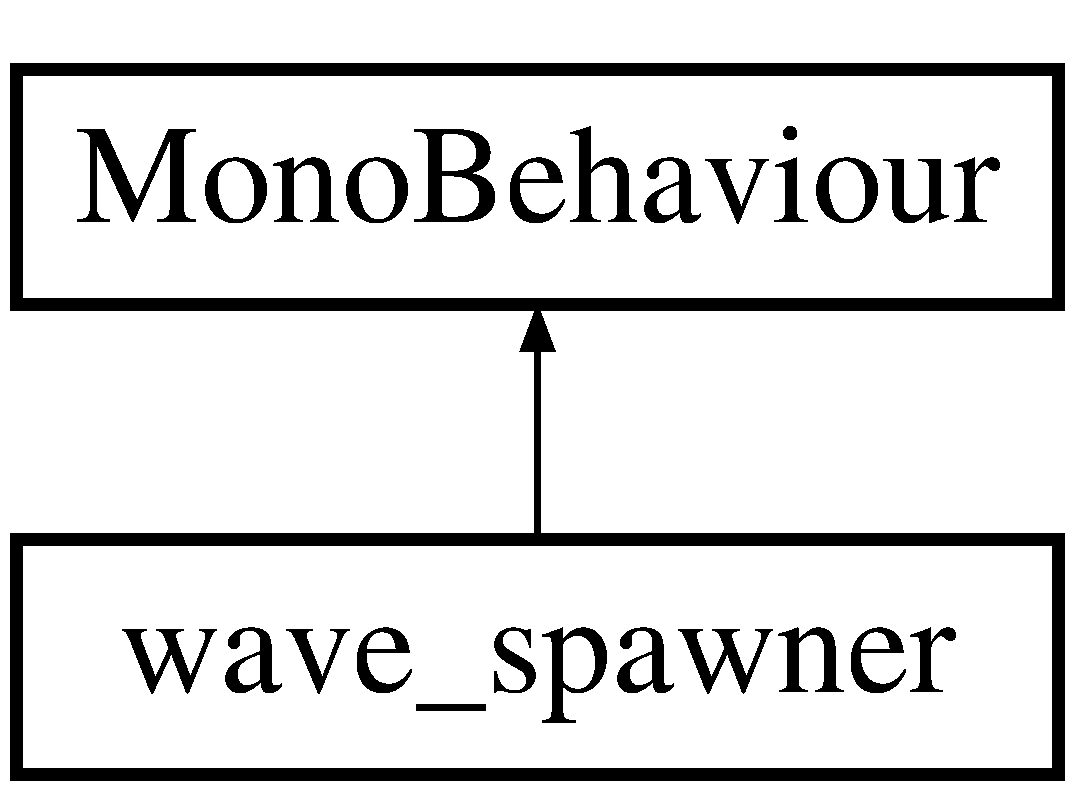
\includegraphics[height=2.000000cm]{classwave__spawner}
\end{center}
\end{figure}
\subsection*{Public Attributes}
\begin{DoxyCompactItemize}
\item 
\mbox{\Hypertarget{classwave__spawner_ab4dc5725df6456980068ee94a159d361}\label{classwave__spawner_ab4dc5725df6456980068ee94a159d361}} 
Transform {\bfseries enemy\+\_\+prefab}
\item 
\mbox{\Hypertarget{classwave__spawner_a1b18aba1e910346fb16de96894d3d4fa}\label{classwave__spawner_a1b18aba1e910346fb16de96894d3d4fa}} 
Transform {\bfseries spawn\+\_\+point}
\item 
\mbox{\Hypertarget{classwave__spawner_abbc823be2179bae1976ed1751abf9c15}\label{classwave__spawner_abbc823be2179bae1976ed1751abf9c15}} 
float {\bfseries time\+\_\+between\+\_\+waves} = 5.\+5f
\item 
\mbox{\Hypertarget{classwave__spawner_a5a53cfa452310466ba0770f00c2911a5}\label{classwave__spawner_a5a53cfa452310466ba0770f00c2911a5}} 
float {\bfseries spawn\+\_\+pause} = 0.\+5f
\item 
\mbox{\Hypertarget{classwave__spawner_a7fed1f46da7e53b59badb80c26e0941c}\label{classwave__spawner_a7fed1f46da7e53b59badb80c26e0941c}} 
Text {\bfseries wave\+\_\+countdown\+\_\+text}
\item 
\mbox{\Hypertarget{classwave__spawner_abf42ed3ce54dbfa0d76c39298513501d}\label{classwave__spawner_abf42ed3ce54dbfa0d76c39298513501d}} 
int {\bfseries wave\+\_\+max} = 10
\item 
\mbox{\Hypertarget{classwave__spawner_a6059e8fd76ba1f7b5b17bdbe80f919b2}\label{classwave__spawner_a6059e8fd76ba1f7b5b17bdbe80f919b2}} 
int {\bfseries testing} = 0
\end{DoxyCompactItemize}
\subsection*{Private Member Functions}
\begin{DoxyCompactItemize}
\item 
void \hyperlink{classwave__spawner_ae049116b14cb20519c1c5a2dc2b824d8}{Update} ()
\item 
I\+Enumerator \hyperlink{classwave__spawner_ad77dc8cd1dbf901d7be2336b5768829e}{Spawn\+\_\+wave} ()
\item 
void \hyperlink{classwave__spawner_a21e2893023c0716bee2f0811eaee7fa2}{Spawn\+\_\+enemy} ()
\end{DoxyCompactItemize}
\subsection*{Private Attributes}
\begin{DoxyCompactItemize}
\item 
\mbox{\Hypertarget{classwave__spawner_a6f2f5e8ba354225136c8c116508ca207}\label{classwave__spawner_a6f2f5e8ba354225136c8c116508ca207}} 
float {\bfseries start\+\_\+time\+\_\+between\+\_\+waves} = 5.\+5f
\item 
\mbox{\Hypertarget{classwave__spawner_af3057e46998da1c5bee5cc59f1bf6287}\label{classwave__spawner_af3057e46998da1c5bee5cc59f1bf6287}} 
float {\bfseries countdown} = 2f
\item 
\mbox{\Hypertarget{classwave__spawner_a8befc58cd3205bc2419130ea673bafbc}\label{classwave__spawner_a8befc58cd3205bc2419130ea673bafbc}} 
int {\bfseries wave\+\_\+index} = 0
\item 
\mbox{\Hypertarget{classwave__spawner_aaca06bce5c3dce2a136ef86051580b9c}\label{classwave__spawner_aaca06bce5c3dce2a136ef86051580b9c}} 
int {\bfseries wave\+\_\+count\+\_\+test} = 0
\item 
\mbox{\Hypertarget{classwave__spawner_a70cfa3a01164c8cd2bb2a7fcad47fd2c}\label{classwave__spawner_a70cfa3a01164c8cd2bb2a7fcad47fd2c}} 
Text {\bfseries wave\+\_\+count\+\_\+test\+\_\+text}
\end{DoxyCompactItemize}


\subsection{Member Function Documentation}
\mbox{\Hypertarget{classwave__spawner_a21e2893023c0716bee2f0811eaee7fa2}\label{classwave__spawner_a21e2893023c0716bee2f0811eaee7fa2}} 
\index{wave\+\_\+spawner@{wave\+\_\+spawner}!Spawn\+\_\+enemy@{Spawn\+\_\+enemy}}
\index{Spawn\+\_\+enemy@{Spawn\+\_\+enemy}!wave\+\_\+spawner@{wave\+\_\+spawner}}
\subsubsection{\texorpdfstring{Spawn\+\_\+enemy()}{Spawn\_enemy()}}
{\footnotesize\ttfamily void wave\+\_\+spawner.\+Spawn\+\_\+enemy (\begin{DoxyParamCaption}{ }\end{DoxyParamCaption})\hspace{0.3cm}{\ttfamily [private]}}

Pre\+: none Post\+: Enemy object created at spawn point return\+: NA \mbox{\Hypertarget{classwave__spawner_ad77dc8cd1dbf901d7be2336b5768829e}\label{classwave__spawner_ad77dc8cd1dbf901d7be2336b5768829e}} 
\index{wave\+\_\+spawner@{wave\+\_\+spawner}!Spawn\+\_\+wave@{Spawn\+\_\+wave}}
\index{Spawn\+\_\+wave@{Spawn\+\_\+wave}!wave\+\_\+spawner@{wave\+\_\+spawner}}
\subsubsection{\texorpdfstring{Spawn\+\_\+wave()}{Spawn\_wave()}}
{\footnotesize\ttfamily I\+Enumerator wave\+\_\+spawner.\+Spawn\+\_\+wave (\begin{DoxyParamCaption}{ }\end{DoxyParamCaption})\hspace{0.3cm}{\ttfamily [private]}}

Pre\+: countdown timer expired Post\+: spawn\+\_\+enemy called for the wave return\+: NA \mbox{\Hypertarget{classwave__spawner_ae049116b14cb20519c1c5a2dc2b824d8}\label{classwave__spawner_ae049116b14cb20519c1c5a2dc2b824d8}} 
\index{wave\+\_\+spawner@{wave\+\_\+spawner}!Update@{Update}}
\index{Update@{Update}!wave\+\_\+spawner@{wave\+\_\+spawner}}
\subsubsection{\texorpdfstring{Update()}{Update()}}
{\footnotesize\ttfamily void wave\+\_\+spawner.\+Update (\begin{DoxyParamCaption}{ }\end{DoxyParamCaption})\hspace{0.3cm}{\ttfamily [private]}}

Pre\+: wave\+\_\+spawned object created Post\+: counter adjusted and if timer has run out, spawn\+\_\+wave called return\+: NA 

The documentation for this class was generated from the following file\+:\begin{DoxyCompactItemize}
\item 
F\+:/\+E\+E\+C\+S448/project3/\+Project3/3\+D-\/\+R\+P\+G/\+Assets/\+Scripts/wave\+\_\+spawner.\+cs\end{DoxyCompactItemize}

\hypertarget{classwaypoints}{}\section{waypoints Class Reference}
\label{classwaypoints}\index{waypoints@{waypoints}}
Inheritance diagram for waypoints\+:\begin{figure}[H]
\begin{center}
\leavevmode
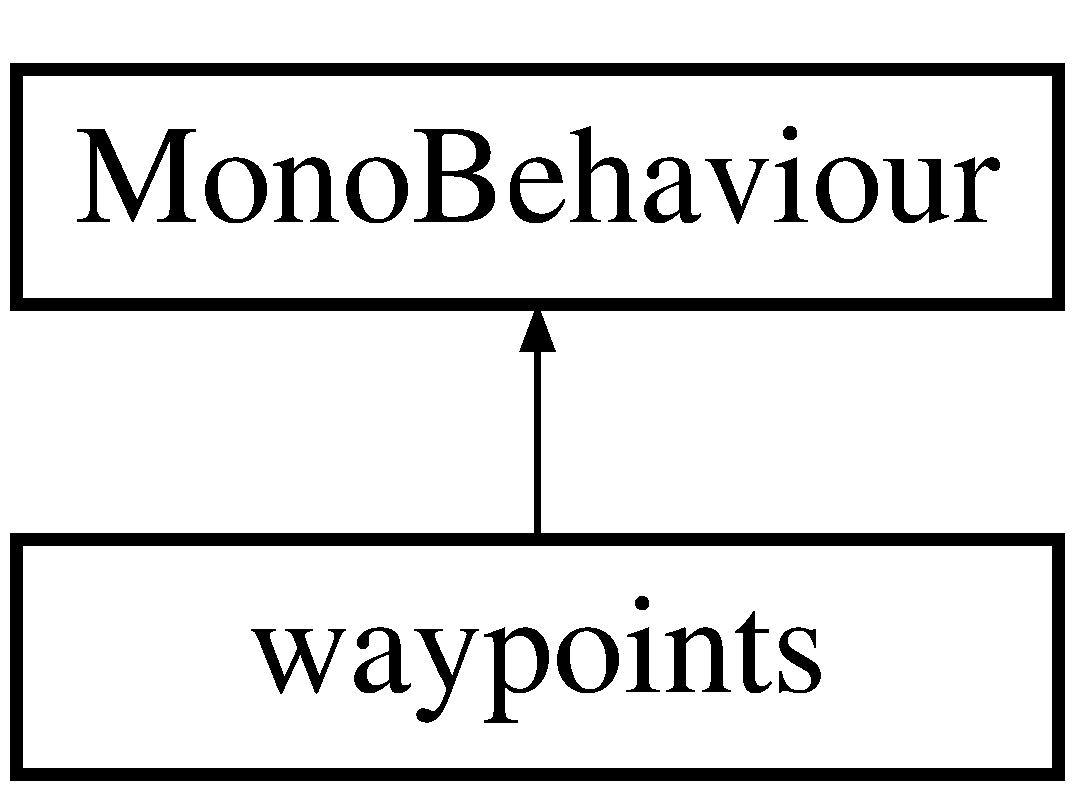
\includegraphics[height=2.000000cm]{classwaypoints}
\end{center}
\end{figure}
\subsection*{Static Public Attributes}
\begin{DoxyCompactItemize}
\item 
\mbox{\Hypertarget{classwaypoints_aeb6c02b5eda032e8ac18c0bc79214cff}\label{classwaypoints_aeb6c02b5eda032e8ac18c0bc79214cff}} 
static Transform \mbox{[}$\,$\mbox{]} {\bfseries points}
\end{DoxyCompactItemize}
\subsection*{Private Member Functions}
\begin{DoxyCompactItemize}
\item 
void \hyperlink{classwaypoints_ab4aab525c65e64319c6857609e1405d7}{Awake} ()
\end{DoxyCompactItemize}


\subsection{Member Function Documentation}
\mbox{\Hypertarget{classwaypoints_ab4aab525c65e64319c6857609e1405d7}\label{classwaypoints_ab4aab525c65e64319c6857609e1405d7}} 
\index{waypoints@{waypoints}!Awake@{Awake}}
\index{Awake@{Awake}!waypoints@{waypoints}}
\subsubsection{\texorpdfstring{Awake()}{Awake()}}
{\footnotesize\ttfamily void waypoints.\+Awake (\begin{DoxyParamCaption}{ }\end{DoxyParamCaption})\hspace{0.3cm}{\ttfamily [private]}}

Pre\+: waypoints object created Post\+: waypoints array created return\+: NA 

The documentation for this class was generated from the following file\+:\begin{DoxyCompactItemize}
\item 
F\+:/\+E\+E\+C\+S448/project3/\+Project3/3\+D-\/\+R\+P\+G/\+Assets/\+Scripts/waypoints.\+cs\end{DoxyCompactItemize}

%--- End generated contents ---

% Index
\backmatter
\newpage
\phantomsection
\clearemptydoublepage
\addcontentsline{toc}{chapter}{Index}
\printindex

\end{document}
